% +------------------------------------------------------------------------+
% | Reference manual chapter: overlay_ref.tex (Map Overlay)
% +------------------------------------------------------------------------+
% | 
% | Package: ovl (Map Overlay)
% | 
% +------------------------------------------------------------------------+

%+----------------------------------------------------------------------------80
%| update log
%|
%| 01 April 2002 - Eti Ezra
%|    Separated from map_overlay.tex (See previous changes in change log there).
%|     
%+----------------------------------------------------------------------------80


% +========================================================================+
%   Introduction
% +========================================================================+
%\clearpage
%\section{Reference Pages for 2D Planar Maps}
%\ccRefLabel{Pm_Ref_intro}

\chapter{2D Map Overlay}
\label{chap:map_overlay_2_ref}
\ccRefLabel{Ovl_Ref_intro}
\subsection*{Introduction}
Given two planar subdivisions $S_1$ and $S_2$, the overlay of 
$S_1$ and $S_2$, denoted by $O(S_1,S_2)$ is the subdivision 
of the plane induced by the edges of $S_1$ and $S_2$.
In this case, $S_1$ and $S_2$ are called the {\em creators} 
of $O(S_1,S_2)$. The overlay of $S_1$ and $S_2$ is represented as the 
arrangement induced by $S_1$ and $S_2$ which maintains information 
regarding its creators, namely, every feature of $O(S_1,S_2)$ holds pointers 
to the respected features from $S_1$ and $S_2$ which caused its creation.
When a feature $f \in O(S_1,S_2)$ is contained in two other features 
$f_1 \in S_1$ and $f_2 \in S_2$, we say that $f_1$ and $f_2$ 
lay {\em above} $f$, alternatively, we say that 
$f$ is {\em below} $f_1$ and $f_2$.

% Every feature in the overlay $O(S_1, S_2)$ maintains the 
% information regarding the features from $S_1$ and $S_2$ laying above it.
% This information is maintained in the basic components of the DCEL, 
% which implies that each face denoted by $f$ of the DCEL contains two pointers 
% to the two faces of $S_1$ and $S_2$  above it. 
% In the same way, each halfedge $e$ contains two pointers to the halfedges 
% from $S_1$ and $S_2$ created it, note that we need two pointers in the 
% case of overlapping curves. 
% Each halfedge $e$ also maintains two pointers to the faces of the creators above it. 
% In some cases such a pointer is simply the face to the side of the halfedge 
% above $e$, and hence, maintaining the face pointer does not add any new information. 
% However, the latter information is necessary when $e$ lays on the interior of a creator face. 
% In such cases we can not access this information through the halfedges of the creators. 
% In most such cases $e$ is a hole in a face of the overlay.
% In the same way, each vertex $v$ of the DCEL contains two pointers to the 
% possibly two vertices of $S_1$ and $S_2$ above it, 
% as well as two pointers to the possibly respected halfedges of $S_1$ and $S_2$ 
% contain it. In some cases a pointer to the creator halfedge can be obtained by 
% accessing one of the halfedges animating from the vertex laying above $v$.
% In this case we pick one such halfedge arbitrarily.
% However, when dealing with cases in which $v$ is an intersection of two edges, 
% we can not simply access this data through a vertex of the creator.
% In addition, $v$ also contains two pointers to the 
% faces of the creators above it. 
% If $v$ is laying on the boundary of some faces of its creators, 
% we choose one such face arbitrarily.
% Maintaining the latter information is necessary 
% in case $v$ lays on the interior of a creator face.
Figure~\ref{OVL_sec:overlay_example} displays an overlay of two given rectangles.

\begin{figure}[h]
    \begin{ccTexOnly}
        \centerline{
           \includegraphics{overlay_example.ps}
           }
    \end{ccTexOnly}
    \caption{Two rectangles (left) and their overlay (right). We denote the subdivision 
       induced by the first rectangle by $S_1$ and the second by $S_2$. 
       The face $f$ of the overlay is below $f_1$ and the unbounded face of $S_2$. 
       The halfedge $e$ of the overlay contains a halfedge pointer to $e_2$ 
       and two faces pointers to $f_1$ and to $f_2$. 
       The vertex $v$ of the overlay points to $v_2$, contains a halfedge 
       pointer to $e_2$ and is lying below $f_1$ and $f_2$.}
    \label{OVL_sec:overlay_example}
\end{figure}

\begin{ccTexOnly}

The subdivision, representing the overlay and its two creators, 
can be either a \ccStyle{Planar_Map} 
(see Chapter~\ref{I1_ChapterPlanarMap}) 
or a \ccStyle{Planar_Map_with_Intersections} 
(see Chapter~\ref{I1_ChapterPmwx}).
%or an {\it arrangement} (see Chapter~\ref{I1_ChapterArrangement_2}).

\subsection*{Software Design}
The \ccc{Map_overlay_2<Subdivision,Notifier>} class 
is a data structure for maintaining 2D map overlay.
The data structure maintains the subdivision obtained by overlaying 
the two creators,
and also contains two pointers to these creators. 
The underlying combinatorial structure is determined by the
(i) {\it Subdivision} which presents the subdivision type of the arrangement 
representing the overlay and its two creators. 
In our usage, {\it Subdivision} is either a \ccStyle{Planar_Map} or, 
a \ccStyle{Planar_Map_With_Intersections}.
% or an a \ccc{Arrangement}.
Notice that the choice of a subdivision type determines the choice 
of a DCEL and a traits class.
(ii) {\it Notifier} is the notifier class used to update the overlay features. 
{\it Notifier} should be a model of the 
\ccc{PlanarMapWithIntersectionsChangeNotification_2} concept.

\subsection*{Map Overlay Algorithms}
The input to our algorithms are two planar subdivisions denoted by $S_1$ and $S_2$ having 
$N$ vertices in total. The overlay of $S_1$ and $S_2$ has $N+k$ vertices, 
while $k$ is the number of intersections between $S_1$ and $S_2$. 
Consequently, the combinatorial complexity of the overlay is quadratic 
in the size of $S_1$ and $S_2$ in the worst case.
We devised and implemented two different algorithms for computing the map-overlay 
of two given planar subdivisions, 
which we refer to as the {\it incremental} algorithm and the {\it sweep-line} algorithm. 
In general, each of these algorithms constructs the overlay by inserting 
the curves of $S_1$ and $S_2$ into the subdivision representing the overlay,
and maintaining within each input curve its corresponding halfedge. 
The latter information is needed when using the notifier in order to
update the creator pointers. 

As shown by our experiments, the sweep-line algorithm is much faster than the incremental 
algorithm. Hence, users are most encouraged to employ the sweep-line algorithm 
when using \ccStyle{Planar_Map} as the subdivision presenting the overlay. 

\subsection*{Map Overlay DCEL}
The \ccc{Map_overlay_default_dcel<Traits,Vertex_base,Halfedge_base,Face_base>}
class is the data structure representing the DCEL of the overlay. 
The basic components of the DCEL of the overlay are built 
on top of the basic components of the \ccStyle{Planar_Map} or 
the \ccStyle{Planar_Map_With_Intersections} 
(depending on the subdivision we choose in order to represent the overlay and its 
two creators).

The additional information, we maintain in these components, is the pointers 
to the creator components.
Each feature of the overlay points to the features of the creators above it.
This information is maintained in the basic components of the DCEL of the overlay.

\subsection*{Map Overlay Notifier}
Updating the DCEL additional attributes is performed by the {\em Notifier} class.
We extend and override the notification functions of the basic {\em Notifier}, defined 
in the \ccc{Planar_Map_2<Dcel,Traits>} package (see Chapter~\ref{I1_ChapterPlanarMap}), 
in order to update the corresponding features constructed by the overlay.  

\subsection*{Boolean Operations:}
The \ccc{Map_overlay_2<Subsection,Notifier>} package
provides an utility for performing boolean operations on planar 
subdivisions.

An object of the \ccc{Boolean_operations_2<Map_overlay>} 
class is initialized with 
two input subdivisions. 
In the initialization step, it constructs the overlay 
of the two input subdivisions. 
By constructing the overlay, all boolean operations, 
on the two input subdivisions, can be easily provided.
The  \ccc{Boolean_operations_2<Map_overlay>} 
class provides methods for 
performing an intersection, union, 
difference and symmetric difference on the two 
input subdivisions. 
The output of such operations are all resulting vertices, 
halfedges and faces.

\subsection*{Polygons Bops:}
One of the most natural usage of 
the \ccc{Map_overlay_2<Subsection,Notifier>} utilities, 
is performing boolean operations on polygons.

The above utility is a straightforward usage of the 
\ccc{Boolean_operations_2<Map_overlay>} 
class. Hence, every operation obtained from the functions 
for boolean operations on polygons can be achieved by 
directly using the \ccc{Boolean_operations_2<Map_overlay>} 
class. 

The goal of providing these functions, is to 
provide a simple interface for users who are 
interested only in boolean operations on 
polygons, rather than boolean operations 
on planar subdivisions of general curves.

In out interface, we provide four function objects 
for all kinds of boolean operations on polygons,
namely, for intersection, union, difference, and 
symmetric difference.

\subsection*{Example of Overlaying Two Subdivisions of Line Segments:}
The following example demonstrates a simple usage of the 
\ccc{Map_overlay_2<Subdivision,Notifier>} package.
In this example we construct two planar maps of line segments. 
Then we construct their overlay when using the sweep-line algorithm, which is 
the default algorithm for the overlay construction. 
After the overlay is constructed, 
we write its corresponding planar map to the 
standard output stream.

\ccIncludeExampleCode{Map_overlay_2/example1.C}
The input of the program is a text file containing two lists of segments, 
each of which represents an input subdivision.
\ccIncludeExampleCode{Map_overlay_2/example1.cin}

The output of the program looks like this:
\ccIncludeExampleCode{Map_overlay_2/example1.cout}

\subsection*{Concepts}
\ccRefConceptPage{MapOverlayDcel_2}\\
\ccRefConceptPage{MapOverlayDcelVertex_2}\\
\ccRefConceptPage{MapOverlayDcelHalfedge_2}\\
\ccRefConceptPage{MapOverlayDcelFace_2}\\
\ccRefConceptPage{MapOverlayAlgorithm_2}\\
\ccRefConceptPage{MapOverlayNotifier_2}\\
\ccRefConceptPage{PolygonBopsTraits_2}\\

\subsection*{Classes}

\ccRefIdfierPage{CGAL::Map_overlay<Subdivision,Notifier>}\\
\ccRefIdfierPage{CGAL::Ovl_dcel<Traits,V,H,F>}\\
\ccRefIdfierPage{CGAL::Ovl_incremental<Subdivision,Notifier>}\\
\ccRefIdfierPage{CGAL::Ovl_sweep<Subdivision,Notifier>}\\
\ccRefIdfierPage{CGAL::Ovl_notifier<Subdivision>}\\
\ccRefIdfierPage{CGAL::Polygons_do_intersect_2<Traits>}\\
\ccRefIdfierPage{CGAL::Polygons_intersection_2<Traits>}\\
\ccRefIdfierPage{CGAL::Polygons_union_2<Traits>}\\
\ccRefIdfierPage{CGAL::Polygons_difference_2<Traits>}\\
\ccRefIdfierPage{CGAL::Polygons_symmetric_difference_2<Traits>}\\

\end{ccTexOnly}    









